\begin{enumerate}
\item Determine the ratio in which the line $2x+y-4=0$ divides the line segment joining the points $A(2,-2)$  and $B(3,7)$.
\item Find a relation between $x$ and $y$ if the points $(x,y), (1,2)$ and $(7,0)$ are collinear.
\item Find the centre of a circle passing through the points $(6,-6), (3,-7)$ and $(3,3)$.
\item The two opposite vertices of a square are $(-1,2)$ and $(3,2)$. Find the coordinates of the two other vertices.
\item The Class X students of a secondary school in Krishinagar have been allotted a rectangular plot of land for their gardening activity. Sapling of Gulmohar are planted on the boundary at a distance of 1m from each other. there is a triangular grassy lawn in the plot as shown in \figref{fig:7.14}. The students are to sow seeds of flowering plants on the remaining area of the plot.
\begin{enumerate}[label=(\roman*)]
\item Taking $A$ as origin, find the coordinates of the vertices of the triangle.
\item What will be tthe coordinates of the vertices of $\triangle PQR$ if $C$ is the origin Also calculate the areas of the triangles in these cases. What do you observe?
\end{enumerate}
\begin{figure}[ht]
\centering
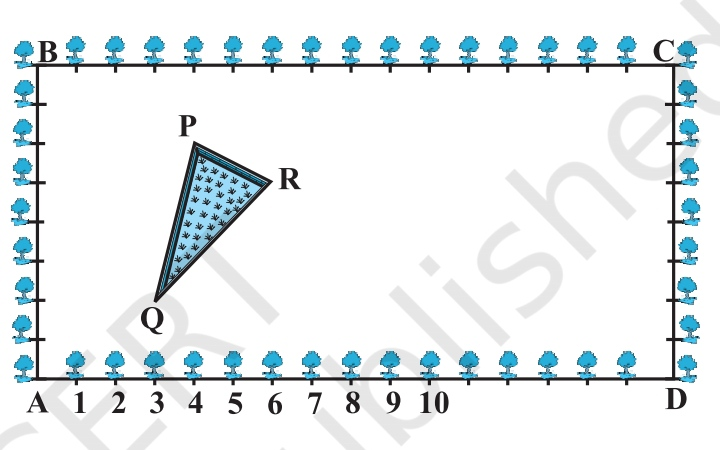
\includegraphics[width=\columnwidth]{chapters/10/figs/7.14.png}
\caption{7.14}
  \label{fig:7.14}
\end{figure}
\item The vertices of a $\triangle ABC$ are $A(4,6), B(1,5)$ and $C(7,2)$. A line is drawn to intersect sides $AB$ and $AC$ at $D$ and $E$ respectively, such that $\frac {AD}{AB}=\frac{AE}{AC}=\frac{1}{4}$. Calculate the area of the $\triangle AD$ and compare it with he area of $\triangle ABC$.
\item Let $A(4,2), B(6,5)$ and $C(1,4)$ be the vertices of $\triangle ABC$.
\begin{enumerate}[label=(\roman*)]
\item The median from $A$ meets $BC$ at $D$. Find the coordinates of the points $D$.
\item Find the coordinates of the point $P$ on $AD$ such that $AP:PD=2:1$.
\item Find the coordinates of points Q and R on medians $BE$ and $CF$ respectively such that $BQ:QE=2:1$ and $CR:RF=2:1$.
\item What do you observe?
\item If $A(x_1,y_1), B(x_2,y_2)$ and $C(x_3,y_3)$ are the vertices of $\triangle ABC$, find the coordinates of the triangle.
\end{enumerate}
\item  $ABCD$ is a rectangle formed by the points  $A(-1,-1), B(-1,4), C(5,4)$ and $D(5,-1)$. $P, Q, R$ and $S$ are the mid points of $AB, BC, CD$ and $DA$ respectively. Is the quadrilateral $PQRS$ a square? a rectangle? or a rhombus? Justify your answer.
\end{enumerate}
